\section{Problema}

% TODO: Agregar sobre la clasificación del problema (lo hago en la introducción ¿Borrar?)

% TODO: Señalar que aunque se habla de clientes pueden ser suministros, ¿Señalar aplicación en ubicación de plantas de biogas de papá?

Se tiene un conjunto de posibles ubicaciones para instalaciones $Z = \{p_1,p_2,...,p_{|Z|}\}$, de las cuales se busca encontrar un subconjunto que maximice el valor de la función objetivo indicada más adelante.

Se tiene un conjunto de ubicaciones de clientes $C = \{c_1,c_2,...,c_{|C|}\}$, cada cliente en $c_i$ tiene asociado un peso $w_i$.

Las ubicaciones pueden ser vectores en $\mathbb{R}^N$, posiciones en una carretera o cualquier espacio métrico $\mathbb{E}$ en que se encuentre definida una métrica de distancia $d : \mathbb{E}^2 \rightarrow \mathbb{R}$ entre cada par de estas.

La función objetivo $\Phi : \mathcal{P}(Z) \rightarrow \mathbb{R}$, que se busca maximizar, está definida para cualquier subconjunto $S$ de $Z$, de la siguiente forma:

\begin{equation}
\Phi(S) = \gamma \cdot |S| + \sum_{i=1}^r \max \left\{0 , \max_{p \in S} \left(
    \alpha \cdot w_i - \beta \cdot w_i \cdot d(c_i,p))
\right) \right\}
\end{equation}

Donde $\gamma$ representa el costo fijo de colocar cada instalación, $\alpha$ representa la ganancia obtenida por cada unidad de peso por cliente conectado y $\beta$ el costo de transporte por cada unidad de peso por cada unidad de distancia. Las funciones $\max$ implican que cada cliente aumentará la función objetivo según su distancia a la instalación más cercana del subconjunto $S$ o ninguna si todas se encuentran muy lejos para obtener una ganancia.

Se llamará \emph{solución} a cualquier subconjunto $S$ de $Z$, sólo son de interés las soluciones, si es que existen, que cumplan con $\Phi(S) > 0$.

\begin{figure}%
    \centering
    \subfloat[Ejemplo de un problema]{{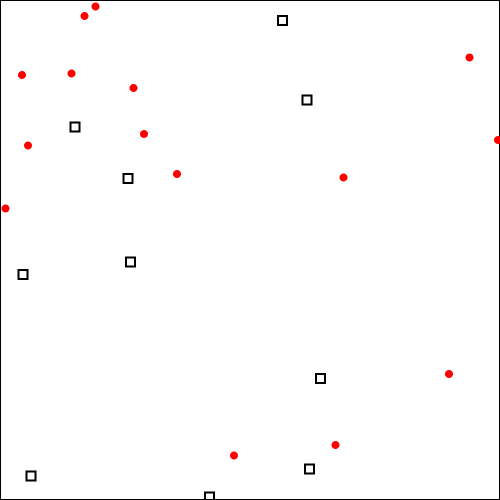
\includegraphics[width=5cm,height=5cm]{small_case_raw.png}}}
    \qquad \qquad \qquad
    \subfloat[Posible solución]{{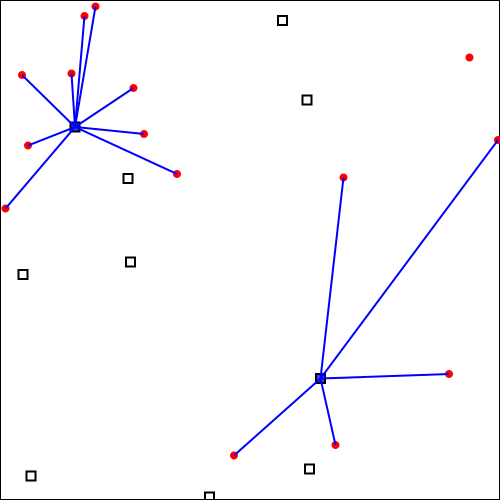
\includegraphics[width=5cm,height=5cm]{small_case_sol.png}}}
    \caption{A la izquierda, ejemplo de un problema, puntos rojos son ubicaciones de clientes, cuadrados son posibles ubicaciones de instalaciones.\\A la derecha una posible solución, cuadrados azules representan subconjunto elegido de ubicaciones de instalaciones, clientes son trabajados por la instalación más cercana o ninguna si todas están muy lejos (tal es el caso del cliente en la esquina superior derecha).}
    \label{fig:algorithm}
\end{figure}

% TODO: Aplicabilidad del modelo a problemas con VAN y costo variable de las instalaciones se puede poner en el costo por unidad.
